\begin{name}
	{\tenchude}{ĐỀ ÔN TẬP SỐ 3}{LỚP TOÁN THẦY PHÁT}{\thoigian}
\end{name}
\setcounter{ex}{0}
\setcounter{bt}{0}
\Opensolutionfile{ans}[ans/ans-Vted-13-2023]
\begin{ex}%[2D2Y4-2]%Câu 1%[Phạm Hoài-Tex-Đề -Vted-2023]%
	Đạo hàm của hàm số $y=3^x$ là
	\choice 
	{$y^{\prime}=\dfrac{3^x}{\ln 3}$}
	{$y^{\prime}=3^x$}
	{$y^{\prime}=x\cdot 3^{x-1}$}
	{\True $y^{\prime}=3^x\cdot \ln 3$}
	\loigiai{Theo định nghĩa đạo hàm của hàm số mũ ta được  $y^{\prime}=3^x\cdot \ln 3$.
	}
\end{ex}	
\begin{ex}%[2H1Y3-2]%Câu 2%[Phạm Hoài-Tex-Đề -Vted-2023]%
	Cho khối lăng trụ có chiều cao là $h=a$ và diện tích đáy $S=3a^2$. Thể tích khối lăng trụ đó bằng
	\choice 
	{\True $V=3a^3$}
	{$V=a^2$}
	{$V=3a^2$}
	{$V=a^3$}
	\loigiai{ Theo công thức thể tích lăng trụ $V=S\cdot h=3a^2\cdot a=3a^3$.}
\end{ex}
\begin{ex}%[2D2B5-2]%Câu 3%[Phạm Hoài-Tex-Đề -Vted-2023]%
	Nghiệm của phương trình $5^{2x-1}=125$ là
	\choice 
	{$x=1$}
	{\True $x=2$}
	{$x=-2$}
	{$x=-1$}
	\loigiai{$5^{2x-1}=125\Leftrightarrow 5^{2x-1}=5^3\Leftrightarrow 2x-1=3\Leftrightarrow 2x=4\Leftrightarrow x=2$.
	}
\end{ex}
\begin{ex}%[2D1B5-4]%Câu 4%[Phạm Hoài-Tex-Đề -Vted-2023]%
	Đồ thị hàm số $y=\dfrac{x+2}{x-1}$ cắt trục tung tại điểm nào dưới đây?
	\choice 
	{$N(-2;0)$}
	{$P(0;2)$}
	{$M(2;0)$}
	{\True $Q(0;-2)$}
	\loigiai{ Đồ thị hàm số cắt trục tung  nên $x=0$.\\
		Khi đó $y=\dfrac{0+2}{0-1}=-2$.\\
		Vậy đồ thị hàm số $y=\dfrac{x+2}{x-1}$ cắt trục tung tại điểm $Q(0;-2)$.
	}
\end{ex}
\begin{ex}%[1D3B4-3]%Câu 5%[Phạm Hoài-Tex-Đề -Vted-2023]%
	Cho cấp số nhân $(u_n)$ có $u_1=\dfrac{1}{2}$, $u_4=-4$. Công bội của cấp số nhân bằng
	\choice 
	{\True $-2$}
	{$\dfrac{3}{2}$}
	{$-\dfrac{3}{2}$}
	{$2$}
	\loigiai{ Ta có $u_4=u_1\cdot q^3\Leftrightarrow -4=\dfrac{1}{2}\cdot q^3\Leftrightarrow q^3=-8\Leftrightarrow q=-2$.\\
		Do đó công bội của cấp số nhân là $q=-2$.
	}
\end{ex}
\begin{ex}%[2D4Y1-2]%Câu 6%[Phạm Hoài-Tex-Đề -Vted-2023]%
	Trong mặt phẳng $Oxy$, số phức $z=2-3i$ có điểm biểu diễn là
	\choice 
	{$P(-2;3)$}
	{\True $M(2;-3)$}
	{$Q(3;-2)$}
	{$N(-3;2)$}
	\loigiai{Số phức $z=2-3i$ có điểm biểu diễn là $M(2;-3)$.
	}
\end{ex}
\begin{ex}%[2H2Y1-1]%Câu 7%[Phạm Hoài-Tex-Đề -Vted-2023]%
	Cho khối nón có đường kính đáy bằng $2a$ và chiều cao bằng $3a$. Thể tích của khối nón bằng
	\choice 
	{$12\pi a^3$}
	{$3\pi a^3$}
	{\True $\pi a^3$}
	{$4\pi a^3$}
	\loigiai{ Ta có bán kính đáy $r=\dfrac{2a}{2}=a$.\\
		$V_{\text{nón}}=\dfrac{1}{3}\cdot S_{\text{đáy}}\cdot h=\dfrac{1}{3}\cdot \pi a^2\cdot 3a=\pi a^3$.\\
		Vậy $V_{\text{nón}}=\pi a^3$.
	}
\end{ex}
\begin{ex}%[2D3B1-1]%Câu 8%[Phạm Hoài-Tex-Đề -Vted-2023]%
	Trong khoảng $(0;+\infty)$, hàm số nào dưới đây \textbf{không} là một nguyên hàm của hàm số $f(x)=\dfrac{1}{x}$?
	\choice 
	{$\ln x+2$}
	{$\ln (2x)$}
	{\True $\ln \dfrac{1}{x}+2$}
	{$\dfrac{1}{2}\ln x^2$}
	\loigiai{\begin{itemize}
			\item $\left(\ln x+2\right)^{\prime}=\dfrac{1}{x}$. Do đó  $\ln x+2$ là một nguyên hàm của hàm số $f(x)=\dfrac{1}{x}$.
			\item $\left(\ln 2x\right)^{\prime }=\dfrac{(2x)^{\prime}}{2x}=\dfrac{1}{x}$. Do đó  $\ln (2x)$ là một nguyên hàm của hàm số $f(x)=\dfrac{1}{x}$.
			\item $\left(\dfrac{1}{2}\ln x^2\right)^{\prime }=\dfrac{1}{2}\left(\ln x^2\right)^{\prime}=\dfrac{1}{2}\dfrac{\left(x^2\right)^{\prime}}{x^2}=\dfrac{1}{x}$. Do đó $\dfrac{1}{2}\ln x^2$ là một nguyên hàm của hàm số $f(x)=\dfrac{1}{x}$.
			\item  $\left(\ln \dfrac{1}{x}+2\right)^{\prime}=\dfrac{\left(\dfrac{1}{x}\right)^{\prime}}{\dfrac{1}{x}}=\dfrac{-\dfrac{1}{x^2}}{\dfrac{1}{x}}=-\dfrac{1}{x}$. Do đó  $\ln \dfrac{1}{x}+2$ không là một nguyên hàm của hàm số $f(x)=\dfrac{1}{x}$.
		\end{itemize}
		
	}
	
\end{ex}
\begin{ex}%[2H3Y3-2]%Câu 9%[Phạm Hoài-Tex-Đề -Vted-2023]%
	Trong không gian $Oxyz$, cho đường thẳng $d\colon \heva{&x=1+t\\&y=2-t\\&z=2t}$. Phương trình chính tắc của $d$ là 
	\choice 
	{$\dfrac{x-1}{1}=\dfrac{y+2}{-1}=\dfrac{z}{2}$}
	{$\dfrac{x+1}{1}=\dfrac{y-2}{-1}=\dfrac{z}{2}$}
	{$\dfrac{x+1}{1}=\dfrac{y+2}{-1}=\dfrac{z}{2}$}
	{\True $\dfrac{x-1}{1}=\dfrac{y-2}{-1}=\dfrac{z}{2}$}
	\loigiai{
		Đường thẳng $d\colon \heva{&x=1+t\\&y=2-t\\&z=2t}$ đi qua điểm $A(1;2;0)$ và có véctơ chỉ phương $\overrightarrow{u}=(1;-1;2)$.\\
		Do đó phương trình chính tắc của đường thẳng $d$ là $\dfrac{x-1}{1}=\dfrac{y-2}{-1}=\dfrac{z}{2}$.
	}
\end{ex}
\begin{ex}%[2D2Y4-1]%Câu 10%[Phạm Hoài-Tex-Đề -Vted-2023]%
	Tập xác định của hàm số $f(x)=x^{-\frac{3}{2}}$ là
	\choice 
	{\True$(0;+\infty)$}
	{ $\mathbb{R}\setminus\{0\}$}
	{$\mathbb{R}$}
	{$[0;+\infty)$}
	\loigiai{
		Cho hàm số  $y=x^{\alpha}$
		\begin{itemize}
			\item $\alpha $ nguyên dương thì $\mathscr{D}=\mathbb{R}$.
			\item $\alpha $ nguyên âm thì $\mathscr{D}=\mathbb{R}\setminus\{0\}$.
			\item $\alpha$ không nguyên thì $x>0$.
		\end{itemize}
		Vì $\alpha =-\dfrac{3}{2}$ không nguyên nên $x>0$. \\Do đó tập xác định của hàm số $f(x)=x^{-\frac{3}{2}}$ là $\mathscr{D}=(0;+\infty)$.
	}
\end{ex}
%==================Câu 11
\begin{ex}%[2D1Y2-2]%[Dự án 12-Vted-2022, Nguyen Huynh]
	Cho hàm số $y=f(x)$ có bảng biến thiên như sau
	\begin{center}
		
\begin{tikzpicture}[>=stealth]
			\tkzTabInit[nocadre=false,lgt=1,espcl=2,deltacl=0.5]
			{$x$/.7 ,$f'(x)$/.7,$f(x)$/2}
			{$-\infty$,$-2$,$0$,$2$,$+\infty$}
			\tkzTabLine{,+,0,-,0,+,0,-} %
			\tkzTabVar{+/$+\infty$,-/$-1$, +/$1$,-/$-1$,+/$+\infty$}
		\end{tikzpicture}
	\end{center}
	Hàm số đã cho đạt cực tiểu tại điểm nào sau đây?
	\choice{\True$x=2$}{$x=0$}{$x=-1$}{$x=1$}
	\loigiai{Dựa theo bảng biến, ta có hàm số $y=f(x)$ đạt cực tiểu tại điểm $x=2$.}
\end{ex}
%==================Câu 12
\begin{ex}%[2H3Y1-3]%[Dự án 12-Vted-2022, Nguyen Huynh]
	Trong không gian $Oxyz$, cho mặt cầu $(S)\colon x^2+y^2+z^2-2x+4y-6z-1=0$. Tâm của mặt cầu $(S)$ có tọa độ là
	\choice
	{$I(-1;2;-3)$}
	{\True$I(1;-2;3)$}
	{$I(-2;4;-6)$}
	{$I(2;-4;6)$}
	\loigiai{
		Mặt cầu $(S)\colon x^2+y^2+z^2-2x+4y-6z-1=0$ có tâm là $I(1;-2;3)$ và bán kính $R=\sqrt{15}$.}
\end{ex}
%==================Câu 13
\begin{ex}%[2D1Y5-1]%[Dự án 12-Vted-2022, Nguyen Huynh]
	\immini{Đường cong trong hình bên là đồ thị của hàm số nào dưới đây?	\choice{\True$y=-x^3+3x-1$}{$y=-x^3-1$}{$y=x^3-3x-1$}{$y=x^3-1$}}	{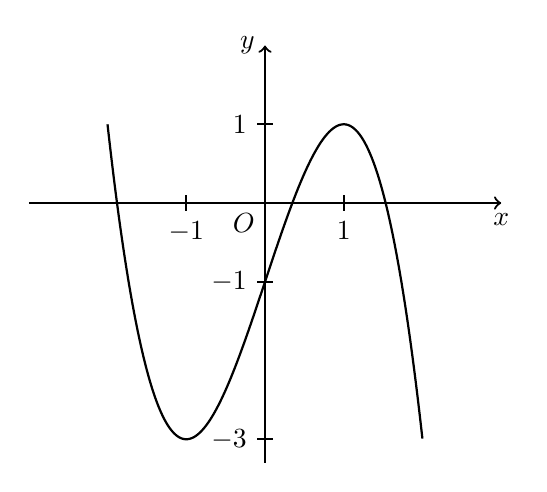
\begin{tikzpicture}[thick,scale=1,nodes={scale=1}]
			\def\a{-1}
			\def\b{0}
			\def\c{3}
			\def\d{-1}
			\def\f(#1){\a*((#1)^3)+\b*((#1)^2)+\c*(#1)+\d}
			\def\xmin{-2}
			\def\xmax{2}
			\def\ymin{-2.3}
			\def\ymax{1}
			\draw[->] (\xmin-1,0)--(\xmax+1,0) node[below] { $x$};
			\draw[->] (0,\ymin-1)--(0,\ymax+1) node[left] { $y$};
			\draw (0,0) node [below left] { $O$};
			\foreach \x in {-1,1}\draw (\x,0.1)--(\x,-0.1) node [below] { $\x$};
			\foreach \y in {-3,-1,1}\draw (0.1,\y)--(-0.1,\y) node [left] { $\y$};
			%	\clip (\xmin,\ymin) rectangle (\xmax,\ymax);
			\draw[thick,smooth,samples=200] plot[domain=\xmin:\xmax] (\x,{\f(\x)});
	\end{tikzpicture}}	
	
	\loigiai{Xét hàm số bậc ba $y=ax^3+bx^2+cx+d$. Dựa vào đồ thị của hàm số, ta có $a<0$ và hàm số $y$ có hai điểm cực trị nên ta chọn $y=-x^3+3x-1$.}
\end{ex}
%==================Câu 14
\begin{ex}%[2D2Y3-2]%[Dự án 12-Vted-2022, Nguyen Huynh]
	Với mỗi số thực $a$, $\log_3(9^a)$ bằng
	\choice{$a$}{$a+2$}{\True$2a$}{$\dfrac{1}{2a}$}
	\loigiai{Ta có $\log_3(9^a)=\log_3(3^{2a})=2a$. }
\end{ex}
%==================Câu 15
\begin{ex}%[2D4Y2-2]%[Dự án 12-Vted-2022, Nguyen Huynh]
	Cho hai số phức $z=2+3i$ và $w=4-5i$. Phần ảo của số phức $z-w$ là
	\choice{$-2i$}{$2$}{\True$8$}{$8i$}
	\loigiai{Ta có $z-w=-2+8i$. Suy ra phần ảo của số phức $z-w$ là $8$. }
\end{ex}
%==================Câu 16
\begin{ex}%[2H1Y3-2]%[Dự án 12-Vted-2022, Nguyen Huynh]
	Cho khối chóp có diện tích đáy $B=12$ và chiều cao $h=6$. Thể tích của khối chóp đã cho bằng
	\choice
	{$72$}
	{\True $24$}
	{$6$}
	{$36$}
	\loigiai{
		Thể tích khối chóp $V=\dfrac{1}{3}Bh=\dfrac{1}{3}\cdot 12 \cdot 6= 24$.
	}
	
\end{ex}
%==================Câu 17
\begin{ex}%[1D2Y2-1]%[Dự án 12-Vted-2022, Nguyen Huynh]
	Với $k, n$ là hai số nguyên dương tùy ý thỏa mãn $k \leq n$, mệnh đề nào sau đây đúng?
	\choice
	{$\mathrm A_n^k=\dfrac{n !}{k !(n-k) !}$}
	{$\mathrm A_n^k=\dfrac{n !}{k !}$}
	{\True $\mathrm A_n^k=\dfrac{n !}{(n-k) !}$}
	{$\mathrm A_n^k=\dfrac{k !(n-k) !}{n !}$}
	\loigiai{
		Công thức $\mathrm A_n^k=\dfrac{n !}{(n-k) !}$.
	}
\end{ex}
%==================Câu 18
\begin{ex}%[2D2Y6-1]%[Dự án 12-Vted-2022, Nguyen Huynh]
	Tập nghiệm của bất phương trình $\log _{\frac{2}{3}}x>2$ là
	\choice
	{\True $\left(0 ; \dfrac{4}{9}\right)$}
	{$\left(\dfrac{4}{9};+\infty\right)$}
	{$\left(\dfrac{4}{3};+\infty\right)$}
	{$\left(0 ; \dfrac{4}{3}\right)$}
	\loigiai{
		Ta có	$\log _{\frac{2}{3}}x>2 \Leftrightarrow 0<x<\left(\dfrac{2}{3}\right)^2\Leftrightarrow 0<x<\dfrac{4}{9}$.
	}
\end{ex}
%==================Câu 19
\begin{ex}%[2H2Y2-1]%[Dự án 12-Vted-2022, Nguyen Huynh]
	Cho mặt cầu có bán kính $r=2$. Diện tích của mặt cầu đã cho bằng
	\choice
	{$\dfrac{16 \pi}{3}$}
	{\True $16 \pi$}
	{$\dfrac{32 \pi}{3}$}
	{$4 \pi$}
	\loigiai{
		Diện tích mặt cầu $S=4\pi r^2=4\pi \cdot 2^2=16\pi$.
	}
\end{ex}
%==================Câu 20
\begin{ex}%[2D1Y4-1]%[Dự án 12-Vted-2022, Nguyen Huynh]
	Tiệm cận ngang của đồ thị hàm số $y=\dfrac{4 x-1}{x+1}$ là đường thẳng có phương trình
	\choice
	{$y=-4$}
	{$y=1$}
	{\True $y=4$}
	{$y=-1$}
	\loigiai{
		Phương trình đường tiệm cận ngang $y= \lim\limits_{x\to \pm \infty}\dfrac{4x-1}{x+1}=4$.
	}
\end{ex}
%%==========Câu 21
\begin{ex}%[Nguyễn Thắng-Dự Án Vted 2023 đề 13]%[2D1Y1-2]
	Cho hàm số $y=f(x)$ có bảng xét dấu như sau
	\begin{center}
		% Cần khai báo \usepackage{tkz-tab}
		
\begin{tikzpicture}
			\tkzTabInit[nocadre=false,lgt=1.2,espcl=2,deltacl=0.5]{$x$/1 ,$f'(x)$/1}
			{$-\infty$ , $-2$ , $0$ , $2$ , $+\infty$}
			\tkzTabLine{  , + , 0 , - , 0 , + , 0 , - }
		\end{tikzpicture}
	\end{center}
	Hàm số đã cho nghịch biến trên khoảng nào dưới đây?
	\choice
	{$(0;+\infty)$}
	{$(-2;2)$}
	{\True $(-2;0)$}
	{$(-\infty;-2)$}
	\loigiai{Dựa vào bảng biến thiên, ta thấy hàm số đã cho nghịch biến trên khoảng $(-2;0)$ và $(2;+\infty)$.
	}
\end{ex}

%%==========Câu 22
\begin{ex}%[Nguyễn Thắng-Dự Án Vted 2023 đề 13]%[2H3Y2-3]
	Trong không gian $Oxyz$, mặt phẳng đi qua $O$ và nhận véc-tơ $\vec{n}=(1;-2;5)$ làm véc-tơ pháp tuyến có phương trình là
	\choice
	{$x+2y-5z=0$}
	{$x+2y-5z+1=0$}
	{\True $x-2y+5z=0$}
	{$x-2y+5z+1=0$}
	\loigiai{
		Mặt phẳng đi qua $O$ và nhận véc-tơ $\vec{n}=(1;-2;5)$ làm véc-tơ pháp tuyến có phương trình là $x-2y+5z=0$.
	}
\end{ex}

%%==========Câu 23
\begin{ex}%[Nguyễn Thắng-Dự Án Vted 2023 đề 13]%[2D1Y2-2]
	\immini[thm]{Cho hàm số $y=ax^4+bx^2+c$ ($a,b,c\in\mathbb{R}$) có đồ thị là đường cong trong hình bên. Điểm cực đại của đồ thị hàm số đã cho là
		\choice[2]
		{$x=0$}
		{\True $M(0;-1)$}
		{$y=-1$}
		{$N(-1;-2)$}}{
		% Đồ thị hàm y=ax^4+bx^2+c. Nếu hệ số lớn cần điều chỉnh hệ trục, vùng lưới, domain và lệnh \clip
		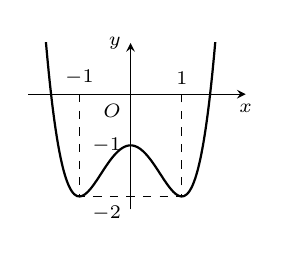
\begin{tikzpicture}[>=stealth,x=1cm,y=1cm,scale=.65]
			\def\a{1} % Hệ số a phải khác 0
			\def\b{-2}
			\def\c{-1}
			\draw[->] (-2,0) -- (2.25,0) node[below] {\scriptsize $x$};
			\draw[->] (0,-2.25) -- (0,1) node[left] {\scriptsize $y$};
			\draw[dashed] (0,0)node[below left]{\scriptsize $O$}
			(-1,0)node[above]{\scriptsize $-1$}|-(0,-2)node[below left]{\scriptsize $-2$}-|(1,0)node[above]{\scriptsize $1$}
			(0,-1)node[left]{\scriptsize $-1$}
			;
			\clip (-2,-2.25)rectangle(2.25,1);
			\draw[thick,samples=150,smooth,domain=-4:4] plot(\x,{\a*(\x)^4+(\b)*(\x)^2+(\c)});
		\end{tikzpicture}	
	}
	\loigiai{
		Dựa vào đồ thị, ta thấy điểm cực đại của đồ thị hàm số là $M(0,-1)$.
	}
\end{ex}

%%==========Câu 24
\begin{ex}%[Nguyễn Thắng-Dự Án Vted 2023 đề 13]%[2D3Y2-1]
	Cho $f$ là hàm số liên tục trên đoạn $[1;2]$. Biết $F$ là nguyên hàm của $f$ trên đoạn $[1;2]$ thỏa
	mãn $F(1)=-2$ và $F(2)=4$. Khi đó $\displaystyle\int\limits_1^2f(x)\mathrm{\,d}x$ bằng
	\choice
	{\True $6$}
	{$2$}
	{$-6$}
	{$-2$}
	\loigiai{
		Ta có $\displaystyle\int\limits_1^2f(x)\mathrm{\,d}x=F(x)\bigg|_1^2=F(2)-F(1)=6$.
	}
\end{ex}

%%==========Câu 25
\begin{ex}%[Nguyễn Thắng-Dự Án Vted 2023 đề 13]%[2D3Y2-1]
	Nếu $\displaystyle\int\limits_0^1f(x)\mathrm{\,d}x=2$ và $\displaystyle\int\limits_1^3f(x)\mathrm{\,d}x=5$ thì $\displaystyle\int\limits_0^3f(x)\mathrm{\,d}x$ bằng
	\choice
	{$10$}
	{$3$}
	{\True $7$}
	{$-3$}
	\loigiai{
		Ta có $\displaystyle\int\limits_0^3f(x)\mathrm{\,d}x=\int\limits_0^1f(x)\mathrm{\,d}x+\int\limits_1^3f(x)\mathrm{\,d}x=2+5=7$.
	}
\end{ex}

%%==========Câu 26
\begin{ex}%[Nguyễn Thắng-Dự Án Vted 2023 đề 13]%[2H3Y1-2]
	Trong không gian $Oxyz$, cho hai véctơ $\vec{u}=(1;-2;3)$ và $\vec{v}=(0;1;-1)$. Khi đó $\vec{u}\cdot\vec{v}$
	bằng
	\choice
	{\True$-5$}
	{$5$}
	{$2\sqrt{7}$}
	{$-2$}
	\loigiai{
		Ta có $\vec{u}\cdot\vec{v}=1\cdot0+(-2)\cdot1+3\cdot(-1)=-5$.
	}
\end{ex}

%%==========Câu 27
\begin{ex}%[Nguyễn Thắng-Dự Án Vted 2023 đề 13]%[2D3B1-1]
	Cho hàm số $f(x)=\mathrm{e}^{2x}+\sin3x$. Khẳng định nào dưới đây đúng?
	\choice
	{$\displaystyle\int f(x)\mathrm{\,d}x=\mathrm{e}^{2x}-\dfrac{1}{3}\cos3x+C$}
	{$\displaystyle\int f(x)\mathrm{\,d}x=\mathrm{e}^{2x}-\cos3x+C$}
	{ $\displaystyle\int f(x)\mathrm{\,d}x=\dfrac{\mathrm{e}^{2x}}{2}+\dfrac{\sin3x}{3}+C$}
	{\True$\displaystyle\int f(x)\mathrm{\,d}x=\dfrac{\mathrm{e}^{2x}}{2}-\dfrac{\cos3x}{3}+C$}
	\loigiai{
		Ta có $\displaystyle\int \left(\mathrm{e}^{2x}+\sin3x\right)\mathrm{\,d}x=\dfrac{\mathrm{e}^{2x}}{2}-\dfrac{\cos3x}{3}+C$.
	}
\end{ex}

%%==========Câu 28
\begin{ex}%[Nguyễn Thắng-Dự Án Vted 2023 đề 13]%[2D1B2-1]
	Hàm số nào dưới đây không có điểm cực trị?
	\choice
	{\True$y=\dfrac{3x-1}{x+1}$}
	{$x^3-x$}
	{$y=x^4-2x^2$}
	{$y=x^2-2x$}
	\loigiai{
		Hàm số $y=\dfrac{3x-1}{x+1}$ có $y'=\dfrac{4}{(x+1)^2}>0,\,\forall x\in\mathbb{R}\backslash\{-1\}$ nên hàm số không có điểm cực trị.
	}
\end{ex}

%%==========Câu 29
\begin{ex}%[Nguyễn Thắng-Dự Án Vted 2023 đề 13]%[2D4B3-2]
	Cho số phức $z$ thỏa mãn $(1+i)\cdot\overline{z}=10+4i$. Phần ảo của $z$ bằng
	\choice
	{$-3$}
	{$7$}
	{\True$3$}
	{$-7$}
	\loigiai{
		Ta có $(1+i)\cdot\overline{z}=10+4i\Leftrightarrow \overline{z}=7-3i$ nên $z=7+3i$.\\
		Phần ảo của $z$ bằng $3$.
	}
\end{ex}
\begin{ex}%[Nguyen Tuan, dự án tex đề VTED lần 2 2023]%[2H1B3-2]
	Cho khối hộp đứng $ABCD.A'B'C'D'$ có tất cả các cạnh bằng $6a$ và $\widehat{BAD}=30^\circ$. Thể tích khối hộp đã cho bằng
	\choice{$36a^3$}{$18a^3$}{$108a^3$}{\True $54a^3$}
	\loigiai{
		\immini
		{
			Diện tích đáy $ABCD$ bằng $S_{ABCD}=\dfrac{1}{2}AB\cdot AD\cdot \sin\widehat{BAD}=\dfrac{1}{2}\cdot 6a\cdot 6a\cdot \dfrac{1}{2}=9a^2$.\\
			Vậy thể tích khối hộp $ABCD.A'B'C'D'$ là
			$$V_{ABCD.A'B'C'D'}=9a^2\cdot 6a=54a^3.$$
		}
		{
			\begin{tikzpicture}[scale=0.7,line join=round,line cap=round,font=\footnotesize,>=stealth]
				\path
				(0,0) coordinate (A)
				(-1,-1) coordinate (B)
				(3,0) coordinate (D)
				($(B)+(D)-(A)$) coordinate (C)
				($(A)+(0,3)$) coordinate (A')
				($(B)+(0,3)$) coordinate (B')
				($(C)+(0,3)$) coordinate (C')
				($(D)+(0,3)$) coordinate (D')
				;
				\draw (C)--(C')--(B')--(B)--(C)--(D)--(D')--(A')--(B') (C')--(D');
				\draw[dashed] (A')--(A)--(B) (A)--(D);
				\foreach \d/\g in {A/-70,B/-120,C/-90,D/-20,A'/90,B'/180,C'/100,D'/20}{
					\draw[fill=black](\d) circle (1pt) +(\g:.35)node{$\d$};}
				
			\end{tikzpicture}
		}
	}
\end{ex}
\begin{ex}%[Nguyen Tuan, dự án tex đề VTED lần 2 2023]%[2D3Y2-1]
	Nếu $\displaystyle\int\limits_0^2 f(x)\mathrm{\,d}x=4$ thì $\displaystyle\int\limits_0^2[3f(x)-2x+1]\mathrm{\,d}x$ bằng
	\choice{\True $10$}{$2$}{$6$}{$14$}
	\loigiai{
		Ta có
		\begin{eqnarray*}
			&& \displaystyle\int\limits_0^2[3f(x)-2x+1]\mathrm{\,d}x\\
			&=& \displaystyle\int\limits_0^2 3f(x)\mathrm{\,d}x+\displaystyle\int\limits_0^2\left(-2x+1\right)\mathrm{\,d}x\\
			&=& 12+\left(-x^2+x\right)\Big|_0^2=10.
		\end{eqnarray*}
	}
\end{ex}
\begin{ex}%[Nguyen Tuan, dự án tex đề VTED lần 2 2023]%[2D1B3-1]
	Trên đoạn $[-2;4]$, hàm số $y=x^3-3x^2-1$ đạt giá trị nhỏ nhất tại điểm nào dưới đây?
	\choice{$x=0$}{$x=2$}{\True $x=-2$}{$x=4$}
	\loigiai{
		Hàm số đã cho liên tục trên đoạn $[-2;4]$.\\
		Ta có $y'=3x^2-6x$, $y'=0\Leftrightarrow \hoac{& x=0\in (-2;4) \\ & x=2\in (-2;4).}$\\
		Ta có $y(-2)=-21$, $y(0)=-1$, $y(2)=-5$, $y(4)=15$.\\
		Vậy $\min\limits_{[-2;4]} y=y(-2)=-21$.
	}
\end{ex}
\begin{ex}%[Nguyen Tuan, dự án tex đề VTED lần 2 2023]%[1D2B5-2]
	Chọn ngẫu nhiên đồng thời hai số từ tập hợp gồm $19$ số nguyên dương đầu tiên. Xác suất để chọn được hai số chẵn bằng
	\choice{$\dfrac{10}{19}$}{\True $\dfrac{5}{19}$}{$\dfrac{4}{19}$}{$\dfrac{9}{19}$}
	\loigiai{
		Trong $19$ số nguyên dương đầu tiên có $10$ số lẻ và $9$ số chẵn.\\
		Số phần tử không gian mẫu: $n(\Omega)=\mathrm{C}_{19}^2$.\\
		Gọi $A$ là biến cố \lq\lq Chọn được hai số chẵn\rq\rq\ .\\
		Suy ra $n(A)=\mathrm{C}_{10}^2$.\\
		Vậy $\mathrm{P}(A)=\dfrac{n(A)}{n(\Omega)}=\dfrac{5}{19}$.
	}
\end{ex}
\begin{ex}%[Nguyen Tuan, dự án tex đề VTED lần 2 2023]%[1H3B2-3]
	\immini{
		Cho hình chóp $S.ABCD$ có tất cả các cạnh bằng nhau (tham khảo hình bên). Góc giữa hai đường thẳng $SC$ và $AB$ bằng
		\choice
		{$90^{\circ}$}
		{\True $60^{\circ}$}
		{$30^{\circ}$}
		{$45^{\circ}$}
	}
	{
		\begin{tikzpicture}[scale=0.8, font=\footnotesize, line join=round, line cap=round, >=stealth]
			\def \cao{3};
			\def \x{3};
			\coordinate[label=below left:$A$] (A) at (0,0);
			\coordinate[label=above right:$D$] (D) at (1,.8);
			\coordinate[label=below right:$B$] (B) at (\x,0);
			\coordinate[label=above right:$C$] (C) at ($(B)-(A)+(D)$);
			\coordinate (O) at ($(D)!.5!(B)$);
			\coordinate[label=above left:$S$] (S) at ($(O)+(90:\cao)$);
			\draw (A)--(B)--(C)--(S)--cycle (S)--(B);
			\draw[dashed] (A)--(D)--(C)--(D)--(S)--(A)--(B);
			\foreach \diem in {A,B,C,D,S} \fill (\diem) circle(1pt);
		\end{tikzpicture}
	}
	\loigiai{
		\immini{
			Vì $AB=BC=CD=DA$ nên đáy $ABCD$ là hình thoi. Suy ra $AB \parallel DC$.\\
			Vậy $(SC,AB)=(SC,DC). \quad (1)$\\
			Xét tam giác $SCD$ có $SD=DC=SC$. Suy ra tam giác $SCD$ đều. $\quad (2)$\\
			Từ $(1)$ và $(2)$ suy ra $(SC,AB)=\widehat{SCD}=60^{\circ}$.
		}
		{
			\begin{tikzpicture}[scale=0.8, font=\footnotesize, line join=round, line cap=round, >=stealth]
				\def \cao{3};
				\def \x{3};
				\coordinate[label=below left:$A$] (A) at (0,0);
				\coordinate[label=above right:$D$] (D) at (1,.8);
				\coordinate[label=below right:$B$] (B) at (\x,0);
				\coordinate[label=above right:$C$] (C) at ($(B)-(A)+(D)$);
				\coordinate (O) at ($(D)!.5!(B)$);
				\coordinate[label=above left:$S$] (S) at ($(O)+(90:\cao)$);
				\draw (A)--(B)--(C)--(S)--cycle (S)--(B);
				\draw[dashed] (A)--(D)--(C)--(D)--(S)--(A)--(B);
				\draw pic[draw,blue,angle radius=3mm] {angle = S--C--D};
				\foreach \diem in {A,B,C,D,S} \fill (\diem) circle(1pt);
				
			\end{tikzpicture}	
		}
	}
\end{ex}

\begin{ex}%[Nguyen Tuan, dự án tex đề VTED lần 2 2023]%[1H3B5-3]
	\immini
	{Cho hình lập phương $ABCD.A'B'C'D'$ có cạnh bằng $2a$ (tham khảo hình bên). Khoảng cách từ $C$ đến mặt phẳng $(BDD'B')$ bằng
		\choice
		{$2\sqrt{2}a$}
		{$2\sqrt{3}a$}
		{\True $\sqrt{2}a$}
		{$\sqrt{3}a$}}
	{\begin{tikzpicture}[font=\footnotesize, line join=round, line cap=round, >=stealth, scale=0.7]
			\def\a{3}
			\def\b{2}
			\def\g{30}
			\def\h{3}
			\path
			(0:0) coordinate (D)
			--++(\g:\b) coordinate (A)
			--++(0:\a) coordinate (B)
			--++(\g-180:\b) coordinate (C)
			\foreach \x in {A,B,C,D}{($(\x)+(90:\h)$) coordinate (\x')}
			($(A)!.5!(C)$) coordinate (O)
			($(A')!.65!(C)$) coordinate (M)
			
			;
			\draw[dashed] (A')--(A)--(B)
			(A)--(D);
			\draw
			(B)--(C)--(C')--(B')--cycle
			(B')--(A')--(D')--(C')
			(C)--(D)--(D')
			;
			\foreach \x/\g in
			{A/150,B/-90,C/-90,D/180,A'/90,B'/90,C'/90,D'/90}
			\fill[black](\x) circle (1pt)
			($(\x)+(\g:3mm)$)node{$\x$}; 
			
	\end{tikzpicture}}
	\loigiai{
		\immini
		{Gọi $O$ là giao điểm của $AC$ và $BD$.\\
			Do $ABCD$ là hình vuông nên ta có $CO\perp BD$.\quad $(1)$\\
			Mặt khác $BB'\perp (ABCD)\Rightarrow BB'\perp CO.$\quad $(2)$\\
			Từ $(1)$ và $(2)$ suy ra $CO\perp (BDD'B')\Rightarrow \mathrm{d}\left(C,(BDD'B')\right)=CO$.\\
			Ta có $CO=\dfrac{AC}{2}=\dfrac{AB\sqrt{2}}{2}=\dfrac{2a\sqrt{2}}{2}=\sqrt{2}a$.\\
			Vậy $\mathrm{d}\left(C,(BDD'B')\right)=\sqrt{2}a$.
		}
		{\begin{tikzpicture}[scale=0.7, font=\footnotesize, line join=round, line cap=round, >=stealth]
				\def\a{3}
				\def\b{2}
				\def\g{30}
				\def\h{3}
				\path
				(0:0) coordinate (D)
				--++(\g:\b) coordinate (A)
				--++(0:\a) coordinate (B)
				--++(\g-180:\b) coordinate (C)
				\foreach \x in {A,B,C,D}{($(\x)+(90:\h)$) coordinate (\x')}
				($(A)!.5!(C)$) coordinate (O)
				($(A')!.65!(C)$) coordinate (M)
				
				;
				\draw[dashed] (A')--(A)--(B)
				(A)--(D)--(B) (A)--(C);
				\draw
				(B)--(C)--(C')--(B')--cycle
				(B')--(A')--(D')--(C')
				(C)--(D)--(D')--(B')
				;
				\foreach \x/\g in
				{A/150,B/-90,C/-90,D/180,A'/90,B'/90,C'/90,D'/90,O/90}
				\fill[black](\x) circle (1pt)
				($(\x)+(\g:3mm)$)node{$\x$}; 
				
		\end{tikzpicture}}
	}
\end{ex}
\begin{ex}%[Nguyen Tuan, dự án tex đề VTED lần 2 2023]%[2H3B2-7]
	Trong không gian $Oxyz$, cho điểm $A(1;-1;2)$ và mặt phẳng $(P) \colon 2x-y+3z+1=0$. Mặt phẳng đi qua $A$ và song song với $(P)$ có phương trình là
	\choice
	{$2x+y+3z+7=0$}
	{$2x+y+3z-7=0$}
	{$2x-y+3z+9=0$}
	{\True $2x-y+3z-9=0$}
	\loigiai{
		Gọi $(Q)$ là mặt phẳng đi qua $A$ và song song với $(P)$.\\
		Vì $(Q) \parallel (P)$ nên phương trình của mặt phẳng $(Q)$ có dạng $2x-y+3z+m=0$, với $m \ne 1$.\\
		Mặt khác, mặt phẳng $(Q)$ đi qua $A$ nên $2\cdot 1-(-1)+3\cdot 2+m=0 \Leftrightarrow m=-9$ (thỏa mãn).\\
		Vậy, mặt phẳng $(Q)$ có phương trình $2x-y+3z-9=0$.
	}
\end{ex}
\begin{ex}%[Nguyen Tuan, dự án tex đề VTED lần 2 2023]%[THPT 2021 - Đợt 2 - 101]%[Tran Quoc]%[2D2B3-2]
	Với $a>0$, đặt $\log_{2}(2a)=b$, khi đó $\log_2\left(8a^4\right)$ bằng
	\choice
	{$4b+7$}
	{$4b+3$}
	{$4b$}
	{\True $4b-1$}
	\loigiai{
		Ta có 
		$$\log_2\left(8a^4\right)=\log_2\dfrac{16a^4}{2}=\log_{2}\dfrac{(2a)^4}{2}=\log_2(2a)^4-\log_22=4\log_2(2a)-1=4b-1.$$
	}
\end{ex}

\begin{ex}%[Nguyễn Hoài Nam, Đề 13]%[2H3B3-2]
	Trong không gian $Oxyz$, cho đường thẳng $(d) \colon \heva{&x=2t\\&y=1+t \\ &z=1-3t}$ và mặt phẳng $(P) \colon 3x-2y+z-1=0$. Đường thẳng $(d')$ đi qua $M(2;1;1)$ vuông góc với $(d)$ và song song với $(P)$ có phương trình là
	\choice
	{\True $(d') \colon \dfrac{x+3}{5}=\dfrac{y+10}{11}=\dfrac{z+6}{7}$}
	{$(d') \colon \dfrac{x-2}{5}=\dfrac{y-1}{-11}=\dfrac{z-1}{-7}$}
	{$(d') \colon \dfrac{x+2}{5}=\dfrac{y-1}{-11}=\dfrac{z+1}{-7}$}
	{$(d') \colon \dfrac{x+2}{5}=\dfrac{y+1}{11}=\dfrac{z+1}{7}$}
	\loigiai{
		Vì $(d')$ song song với $(P)$ và vuông góc với $d$ nên VTCP của $(d')$ là $\overrightarrow{u}_{d'}=\left[\overrightarrow{u}_{d},\overrightarrow{n}_{P}\right]=(-5;-11;-7)=-1(5;11;7)$.\\
		Hơn nữa $(d')$ đi qua điểm $M(2;1;1)$ nên $(d') \colon \dfrac{x+3}{5}=\dfrac{y+10}{11}=\dfrac{z+6}{7}$.
	}
\end{ex}
\begin{ex}%[Nguyễn Hoài Nam, Đề 13]%[2H2K1-2]
	Cho một hình trụ mà khi trải mặt xung quanh của nó lên một mặt phẳng ta thu được một hình vuông có độ dài cạnh bằng $4 \pi$. Khi cắt hình trụ đó bởi mặt phẳng song song và cách trục hình trụ một khoảng bằng $1$ ta thu được thiết diện có diện tích bằng
	\choice
	{$8\sqrt{15} \pi$}
	{\True $8 \sqrt{3} \pi$}
	{$8\pi$}
	{$16 \pi$}
	\loigiai{
		\immini{Mặt xung quanh của trụ khi cắt theo một đường sinh và trải lên một mặt phẳng ta thu được hình chữ nhật kích thước  $2\pi r \times h \Rightarrow h=2\pi r=4\pi \Rightarrow r=2$.\\
			Khi cắt hình trụ đó bởi mặt phẳng song song và cách trục hình trụ một khoảng $x=1$ thu được thiệt diện là hình chữ nhật có diện tích bằng $2\sqrt{r^2-x^2} \cdot h=2\sqrt{2^2-1^2}\cdot 4\pi =8\sqrt{3}\pi$.}
		{
			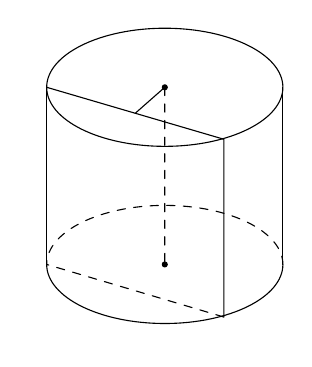
\begin{tikzpicture}[scale=.75,font=\footnotesize, line join=round, line cap=round, >=stealth]
				%\draw[thin,color=gray!50] (0,0) grid (5,5);
				%\draw[-, color=black] (4,0)--(4,1.45);
				\draw[](0,3) arc (0:360:2 and 1);
				%\draw plot [smooth, tension=2] coordinates {(-2,-1) (0,1.3) (-2,1)};
				\draw[dashed] (0,0) arc (0:180:2 and 1);
				\draw(-4,0) arc (180:360:2 and 1);
				\draw (-4,0)--(-4,3) (0,0)--(0,3);
				\filldraw (-2,0) circle(1.2pt);  
				\filldraw (-2,3) circle(1.2pt);  
				\draw[dashed] (-1,-0.89)--(-4,0) (-2,3)--(-2,0);
				\draw(-4,3)--(-1,2.12)--(-1,-0.89);
				\draw(-2.5,2.56)--(-2,3);
				\node[right] at (-2,3) {};
				\node[above left] at (-4,3) {};
				\node[right] at (-2,0) {};
				\node[above] at (-1,2.1) {};
				\node[right] at (-1,-1.1) {};
				\node[above left] at (-4,-0.9) {};
		\end{tikzpicture}}
	}
\end{ex}
\begin{ex}%[Nguyễn Hoài Nam, Đề 13]%[2D2G6-2]
	Có bao nhiêu số nguyên dương $m$ sao cho có ít nhất $10$ số nguyên $x$ thỏa mãn $(x-m)\sqrt{2-\log(4x)}\ge 0$?
	\choice
	{$10$}{\True $16$}{$15$}{$0$}
	\loigiai{
		\begin{eqnarray*}
			(x-m)\sqrt{2-\log(4x)}\ge 0. \quad (1)
		\end{eqnarray*}
		Điều kiện: $2-\log(4x)\ge 0\Leftrightarrow 0<x\le 25$. Ta chỉ xét với $m\ge 1$.
		\begin{itemize}
			\item TH1: $2-\log(4x)=0\Leftrightarrow x=25$ luôn thỏa mãn bất phương trình.
			\item TH2: $2-\log(4x)>0\Leftrightarrow 0<x<25\Rightarrow (1) \Leftrightarrow x-m\ge 0\Leftrightarrow x\ge m $.
			\begin{itemize}
				\item[+] Nếu $m\ge 25\Rightarrow x=25$ không thõa mãn.
				\item[+] Nếu $1\le m<25\Rightarrow x\in [m;25]$ chứa ít nhất 10 số nguyên $x$ là các số $25$, $24,\ldots$, $16\Leftrightarrow m\le 16$\\
				$\Rightarrow m\in \{1,2,\ldots,16\}$.
			\end{itemize}
		\end{itemize}
	}
\end{ex}
\begin{ex}%[Nguyễn Hoài Nam, Đề 13]%[2H3K3-7]
	Trong không gian $Oxyz$, mặt phẳng chứa đường thẳng $d \colon \dfrac{x-2}{1}=\dfrac{y-1}{2}=\dfrac{z}{-1}$  và cắt các trục tọa độ $Ox$, $Oy$ lần lượt tại $A$, $B$ sao cho đường thẳng $AB$ vuông góc với $d$ là
	\choice
	{$2x-y-3=0$}
	{$x+2y+5z-5=0$}
	{\True $x+2y+5z-4=0$}
	{$x+2y-z-4=0$}
	\loigiai{ Gọi $(P) \cap Ox=A(a;0;0)$, $(P) \cap Oy=B(0;b;0)$. Suy ra $\overrightarrow{AB}=(-a;b;0)$.\\
		Véc-tơ chỉ phương của $d$ là $\overrightarrow{u}_d=(1;2;-1)$.\\
		Vì $AB$ vuông góc với $d$ nên
		$$\overrightarrow{AB} \cdot \overrightarrow{u}_d=0 \Leftrightarrow -a+2b=0 \Leftrightarrow a=2b.$$
		Khi đó $\overrightarrow{AB}=(-2b;b;0)$ cùng phương với $\overrightarrow{u}=(-2;1;0)$. \\
		Ta có $\heva{& AB \subset (P)\\&d \subset (P)}.$ Suy ra  véc-tơ pháp tuyến của $(P)$ là $\overrightarrow{n}_{(P)}=\left[ \overrightarrow{u},\overrightarrow{u}_d \right]=(-1;-2;-5)$. \\
		$(P)$ qua điểm $M(2;1;0) \in d$ suy ra $(P) \colon x+2y+5z-4=0.$
	}
\end{ex}
\begin{ex}%[Nguyễn Hoài Nam, Đề 13]%[2D4G5-1]
	Gọi $S$ là tập tất cả các số phức $z$ thỏa mãn $z\cdot \overline{z}=|z+\overline{z}|$. Xét hai số phức $z_1,z_2\in S$ sao cho $|z_1-z_2|=1$, số phức $z_1$ có phần thực dương và số phức $z_2$ có phần thực âm. Giá trị lớn nhất của $P=|z_1-3i|^2+|z_2-3i|^2$ bằng
	\choice{$2+2\sqrt{30}$}{$30+2\sqrt{10}$}{\True $20+6\sqrt{3}$}{$22+4\sqrt{10}$}
	\loigiai{
		Đặt $z=x+yi$, $(x,y\in \mathbb{R})$, suy ra $$x^2+y^2=\left|(x+yi)+(x-yi)\right|\Leftrightarrow x^2+y^2=2|x|\Leftrightarrow \hoac{&x^2+y^2=2x\\&x^2+y^2=-2x.}$$
		Vậy tập hợp các điểm biểu diễn số phức $z$ thuộc hai đường tròn $\left(\mathscr{C}_1\right)$ và $\left(\mathscr{C}_2\right)$ lần lượt có tâm $I_1(1;0)$, $R_1=1$ và $I_2(-1;0)$, $R_2=1$. Gọi $M$, $A$, $B$ lần lượt là điểm biểu diễn của các số phức $3i$, $z_1$, $z_2$. Do số phức $z_1$ có phần thực dương nên $A\in \left(\mathscr{C}_1\right)$ và số phức $z_2$ có phần thực âm nên $B\in \left(\mathscr{C}_2\right)$. 
		\begin{center}
			\begin{tikzpicture}[scale=1, font=\footnotesize, line join=round, line cap=round, >=stealth]
				\draw[-stealth] (-3,0)--(3,0) node[below] {$x$};
				\draw[-stealth] (0,-1.5)--(0,4) node[right] {$y$};
				\path 
				(-1,0) coordinate (I_2)
				(1,0) coordinate (I_1) 
				(0,0) coordinate (O)
				(0,3) coordinate (M)
				(I_2)++(70:1) coordinate (B)
				(I_1)++(130:1) coordinate (A)
				($(A)!0.5!(B)$) coordinate (E)
				(0,3) coordinate (M);
				\draw (I_1) circle (1) (I_2) circle (1);
				\draw (M)--(B)--(A)--cycle (M)--(E);
				\foreach \i/\j in {I_1/-90, I_2/-90, O/-135, A/-30, B/-120, E/120, M/180} \fill (\i) circle (1pt) ++ (\j:0.3) node {$\i$};
			\end{tikzpicture}
		\end{center}
		Ta có $P=MA^2+MB^2=2ME^2+\dfrac{1}{2}AB^2=2ME^2+\dfrac{1}{2}$, trong đó $E$ là trung điểm $AB$.\\
		Ta có $ME\leq MO+OE=2+OE$ và $\left|\overrightarrow{I_1A}\right|=\left|\overrightarrow{I_2B}\right|=\left|\overrightarrow{AB}\right|=1$, ta sẽ phân tích $\overrightarrow{AB}$, $\overrightarrow{OE}$ theo $\overrightarrow{I_1A}$ và $\overrightarrow{I_2B}$. \\
		Ta lại có $$1=\left|\overrightarrow{AB}\right|=\left|\overrightarrow{I_1B}-\overrightarrow{I_1A}\right|=\left|\overrightarrow{I_1I_2}-\left(\overrightarrow{I_1A}-\overrightarrow{I_2B}\right)\right|\geq \left|\overrightarrow{I_1I_2}\right|-\left|\overrightarrow{I_1A}-\overrightarrow{I_2B}\right|\Rightarrow \left|\overrightarrow{I_1A}-\overrightarrow{I_2B}\right|\geq 1.$$
		Khi đó
		\begin{align*}
			2OE&=\left|2\overrightarrow{OE}\right|=\left|\overrightarrow{OA}+\overrightarrow{OB}\right|=\left|\overrightarrow{I_1A}-\overrightarrow{I_1O}+\overrightarrow{I_2B}-\overrightarrow{I_2O}\right|=\left|\overrightarrow{I_1A}+\overrightarrow{I_2B}\right|\\
			&=\sqrt{2\left(\left|\overrightarrow{I_1A}\right|^2+\left|\overrightarrow{I_2B}\right|^2\right)-\left|\overrightarrow{I_1A}-\overrightarrow{I_2B}\right|^2}\leq \sqrt{2(1^2+1^2)-1^2}=\sqrt{3}.
		\end{align*}
		Suy ra $$P\leq 2\left(3+\dfrac{\sqrt{3}}{2}\right)^2+\dfrac{1}{2}=20+6\sqrt{3}.$$
		Dấu \lq\lq=\rq\rq\ khi và chỉ khi $$\heva{&\overrightarrow{I_1A}-\overrightarrow{I_2B}=\dfrac{1}{2}\overrightarrow{I_1I_2}=(-1;0)\\&2\overrightarrow{OE}=\overrightarrow{I_1A}+\overrightarrow{I_2B}=-\dfrac{\sqrt{3}}{3}\overrightarrow{OM}=(0;-\sqrt{3}).}$$
		Suy ra, $\overrightarrow{I_1A}=\left(-\dfrac{1}{2};-\dfrac{\sqrt{3}}{2}\right)$, $\overrightarrow{I_2B}=\left(\dfrac{1}{2};-\dfrac{\sqrt{3}}{2}\right)\Rightarrow A\left(\dfrac{1}{2};-\dfrac{\sqrt{3}}{2}\right)$, $B\left(-\dfrac{1}{2};-\dfrac{\sqrt{3}}{2}\right)$.\\
		Lưu ý: Một cách tương tự ta có $$ME\geq MO-OE=3-OE\geq 3-\dfrac{\sqrt{3}}{2}\Rightarrow P\geq 2\left(3-\dfrac{\sqrt{3}}{2}\right)^2+\dfrac{1}{2}=20-6\sqrt{3}.$$}
\end{ex}
\begin{ex}%[Nguyễn Hoài Nam, Đề 13]%[2D3K1-3]
	Cho hàm số $f(x)$ có đạo hàm $f'(x)=36x(1+\ln x )$, $\forall x\in (0;+\infty)$ và $f(1)=9$. Gọi $F$ là một nguyên hàm của $f$ trên $(0;+\infty)$ sao cho $F(1)=1$, khi đó $F(\mathrm{e})$ bằng
	\choice
	{$7\mathrm{e}^3+9\mathrm{e}-9$}
	{\True $7\mathrm{e}^3$}
	{$27\mathrm{e}^2-8$}
	{$27\mathrm{e}^2$}
	\loigiai{
		\textbf{Cách 1:} Ta có 
		\allowdisplaybreaks
		\begin{eqnarray*}
			f(x) &=& \displaystyle\int f'(x) \mathrm{\,d}x \\
			&=& \displaystyle\int 36x(1+\ln x) \mathrm{\,d}x\\
			&=& \displaystyle\int 36x \mathrm{\,d}x + \displaystyle\int 36x \ln x \mathrm{\,d}x \\
			&=& 18x^2 + \displaystyle\int \ln x \mathrm{\,d}(18x^2)\\
			&=& 18x^2 + 18x^2 \ln x - \displaystyle\int 18x^2 \cdot \dfrac{1}{x} \mathrm{\,d}x\\
			&=& 18x^2 + 18x^2 \ln x - 9x^2 + C\\
			&=& 9x^2 + 18x^2 \ln x + C.
		\end{eqnarray*}
		Vì $f(1)=9 \Rightarrow C=0 \Rightarrow f(x)=9x^2 + 18x^2\ln x$.\\
		Do đó $F(\mathrm{e}) = F(1) + \displaystyle\int\limits_{1}^{\mathrm{e}} f(x)\mathrm{\,d}x = 1+\displaystyle\int\limits_{1}^{\mathrm{e}} (9x^2 + 18x^2 \ln x) \mathrm{\,d}x = 7\mathrm{e}^3$.\\
		\textbf{Cách 2:} Ta có 
		\allowdisplaybreaks
		\begin{eqnarray*}
			F(\mathrm{e}) &=& F(1) + \displaystyle\int\limits_{1}^{\mathrm{e}} f(x)\mathrm{\,d}x \\
			&=& 1 + \displaystyle\int\limits_{1}^{\mathrm{e}} f(x) \mathrm{\,d}x \\
			&=& 1 + xf(x)\Bigg|_{1}^{\mathrm{e}} - \displaystyle\int\limits_{1}^{\mathrm{e}} x f'(x) \mathrm{\,d}x \\
			&=& 1 + \mathrm{e}f(\mathrm{e}) - f(1) - \displaystyle\int\limits_{1}^{\mathrm{e}} xf'(x) \mathrm{\,d}x\\
			&=& 1 + \mathrm{e}\left[ f(1) + \displaystyle\int\limits_{1}^{\mathrm{e}} f'(x) \mathrm{\,d}x  \right] - f(1) - \displaystyle\int\limits_{1}^{\mathrm{e}} xf'(x) \mathrm{\,d}x\\
			&=& 1 + \mathrm{e}\left[ 9 + \displaystyle\int_{1}^{\mathrm{e}} 36x(1+\ln x)\mathrm{\,d}x \right] - 9 - \displaystyle\int_{1}^{\mathrm{e}} 36x^2 (1+\ln x) \mathrm{\,d}x \\
			&=& 7\mathrm{e}^3.
		\end{eqnarray*}
		\textbf{Cách 3:} Ta có 
		\allowdisplaybreaks
		\begin{eqnarray*}
			F(\mathrm{e}) &=& F(1) + \displaystyle\int\limits_{1}^{\mathrm{e}} f(x) \mathrm{\,d}x\\
			&=& 1 + \displaystyle\int\limits_{1}^{\mathrm{e}} f(x) \mathrm{\,d}x\\
			&=& 1 + \displaystyle\int\limits_{1}^{\mathrm{e}} f(x) \mathrm{\,d}(x-\mathrm{e}) \\
			&=& 1 + (x-\mathrm{e})f(x)\Bigg|_{1}^{\mathrm{e}} - \displaystyle\int\limits_{1}^{\mathrm{e}} (x-\mathrm{e})f'(x) \mathrm{\,d}x\\
			&=& 1 - 9(1-\mathrm{e}) - \displaystyle\int\limits_{1}^{\mathrm{e}} (x-\mathrm{e})36x(1+\ln x) \mathrm{\,d}x  \\
			&=& 7\mathrm{e}^3.
		\end{eqnarray*}
	}
\end{ex}
\begin{ex}%[Nguyễn Hoài Nam, Đề 13]%[2D1K5-3]
	Cho hàm số bậc ba $f(x)$ có bảng biến thiên như hình vẽ sau
	\begin{center}
		
\begin{tikzpicture}
			\tkzTabInit[nocadre=false,lgt=1.2,espcl=2.5,deltacl=0.6]
			{$x$ /0.6,$y’$ /0.6,$y$ /2}
			{$-\infty$,$0$,$2$,$+\infty$}
			\tkzTabLine{,+,0,-,0,+,}
			\tkzTabVar{-/$-\infty$,+/$3$,-/$-1$,+/$+\infty$}
		\end{tikzpicture}
	\end{center}
	Số nghiệm thực phân biệt của phương trình $f^2(x)- \left[f(f(x))+2\right]f(x)+2f\left(f(x)\right)=0$ là
	\choice
	{$7$}
	{$12$}
	{\True $10$}
	{$9$}
	\loigiai{
		Đặt $t=f(x)$. Khi đó ta có 
		\begin{eqnarray*}
			t^2 - \left[(f(t)+2)\right]t+2f(t)=0 \quad (1)
		\end{eqnarray*}
		Đồ thị hàm số $f(x)=ax^3+bx^2+cx+d$ có hai điểm cực trị là $A(0;3)$ và $B(2;-1)$ nên 
		\begin{eqnarray*}
			\heva{&f(0)=3\\&f(2)=-1\\&f'(0)=0\\&f'(2)=0} \Leftrightarrow \heva{&d=3\\&8a+4b+2c+d=-1\\&c=0\\&12a+4b+c=0} \Leftrightarrow \heva{&a=1\\&b=-3\\&c=0\\&d=3.}
		\end{eqnarray*}
		Suy ra $f(x)=x^3-3x^2+3$. Khi đó 
		\begin{eqnarray*}
			(1) \Leftrightarrow t^2 - \left(t^3-3t^2+5\right)t+2\left(t^3-3t^2+3\right)=0 \Leftrightarrow -t^4+5t^3-5t^2-5t+6 \Leftrightarrow \hoac{&t=-1\\&t=1\\&t=2\\&t=3} \Leftrightarrow \hoac{&f(x)=-1\Rightarrow \text{ có $2$ nghiệm}\\&f(x)=1\Rightarrow \text{ có $3$ nghiệm}\\&f(x)=2\Rightarrow \text{ có $3$ nghiệm}\\&f(x)=3\Rightarrow \text{ có $2$ nghiệm}.}
		\end{eqnarray*}
		Vậy phương trình đã cho có tất cả $10$ nghiệm.
	}
\end{ex}

%%==========Câu 45
\begin{ex}%[Paul Hieu Nguyen-Dự Án Vted 2023 đề 13]%[2D4K4-1]%Câu 45
	Trên tập các số phức, xét phương trình $z^2+2mz+n^2+1=0$ ($m$, $n$ là tham số thực). Có bao nhiêu cặp số $(m; n)$ sao cho phương trình có hai nghiệm phức $z_1$, $z_2$ sao cho các điểm biểu diễn số phức $z_0=-1$, $z_1$, $z_2$ là ba đỉnh của một tam giác đều có độ dài cạnh bằng $2$?
	\choice
	{$3$}
	{$2$}
	{$6$}
	{\True $4$}
	\loigiai{
		Ta có $\Delta'=m^2-n^2-1$. Gọi $A$, $B$, $C$ lần lượt là điểm biểu diễn của $z_1$, $z_2$ và $z_0$.\\
		\textbf{TH1:} Nếu $\Delta'\geq 0 \Rightarrow z_1$, $z_2 \in \mathbb{R}\Rightarrow A$, $B$, $C \in O x \Rightarrow A$, $B$, $C$ không tạo thành tam giác (loại).\\
		\textbf{TH2:} Nếu $\Delta'<0 \Leftrightarrow m^2-n^2-1<0$ thì \\ $z_1=-m-\sqrt{n^2+1-m^2}\cdot i$; $z_2=-m+\sqrt{n^2+1-m^2}\cdot i$\\ $\Rightarrow A\left(-m ;-\sqrt{n^2+1-m^2}\right)$, $B\left(-m ; \sqrt{n^2+1-m^2}\right)$.\\
		Khi đó $A$, $B$, $C$ là ba đỉnh của một tam giác đều có độ dài cạnh bằng $2$ khi\\
		$\begin{aligned}
			& CA=CB=AB=2 \Leftrightarrow \sqrt{(m-1)^2+n^2+1-m^2}=2 \sqrt{n^2+1-m^2}=2 \\
			& \Leftrightarrow\left\{\begin{aligned}
				& n^2+1-m^2= 1\\
				& (m-1)^2=3
			\end{aligned}\Leftrightarrow \left\{\begin{aligned}
				& n=\pm m \\
				& (m-1)^2=3
			\end{aligned}\Leftrightarrow \left\{\begin{aligned}
				& n=\pm m \\
				& m=1\pm\sqrt{3}.
			\end{aligned}\right.\right.\right.
		\end{aligned}$\\
		Vậy có $4$ cặp số $(m;n)$ thỏa bài toán.
	}
\end{ex}
%%==========Câu 46
\begin{ex}%[Paul Hieu Nguyen-Dự Án Vted 2023 đề 13]%[2D3G3-1]%Câu 46
	\immini{Cho hàm số bậc bốn $f(x)$ có đồ thị của $f(x)$, $f'(x)$ như hình vẽ bên. Gọi $S_1$ và $S_2$ là diện tích của hai hình phẳng được gạch trong hình vẽ. Khi $S_1=1$ thì $S_2$ bằng
		\choice
		{\True $\dfrac{104}{23}$}
		{$\dfrac{70}{23}$}
		{$\dfrac{57}{23}$}
		{$\dfrac{84}{23}$}
	}
	{
		\begin{tikzpicture}[font=\footnotesize,line join=round,line cap=round,>=stealth,scale=.8]
			\tikzset{declare function={xmin=-6;xmax=1;ymin=-1.5;ymax=3;
					a=1/4;b=7/2;c=69/4;d=35;ee=25;
					f(\x)=a*(\x)^4+b*(\x)^3+c*(\x)^2+d*(\x)+ee;
					g(\x)=4*a*(\x)^3+3*b*(\x)^2+2*c*(\x)+d;
				}
			}
			\draw[->](xmin,0)--(xmax,0); \draw(xmax-.1,0) node[below]{$x$};
			\draw[->](0,ymin)--(0,ymax); \draw(0,ymax-.12) node[left]{$y$};
			\draw (0,0)+(-135:.25)node[scale=.9]{$O$};
			\clip(xmin,ymin) rectangle (xmax,ymax);
			\fill[pattern=north west lines,smooth,samples=100,domain=-5:-4] plot (\x,{f(\x)})--plot (\x,{g(\x)});
			\fill[pattern=north west lines,smooth,samples=100,domain=-4:-2] plot (\x,{f(\x)})--plot (\x,{g(\x)});
			\draw[domain=-6:-1,smooth,samples=100] plot(\x,{f(\x)}) plot(\x,{g(\x)});
			\fill[black](-5,0) circle (1pt)+(-150:.45)node[scale=.85]{$-5$};
			\fill[black](-2,0) circle (1pt)+(-50:.3)node[scale=.85]{$-2$};
			\fill[black](-4,{f(-4)}) circle (1pt);
			\draw[->] (-4.5,0.7)--(-5,1.5) node[above,scale=.85]{$S_1$};
			\draw[->] (-3.3,0.66)--(-2.8,1.6) node[above,scale=.85]{$S_2$};
		\end{tikzpicture}
	}
	\loigiai{
		Có $f(x)=a(x+5)^2(x+2)^2$, $\left(\displaystyle\lim\limits _{x \rightarrow +\infty}f(x)=+\infty \Rightarrow a>0\right)$.\\
		Suy ra
		$f'(x)=a\left[2(x+5)(x+2)^2+2(x+2)(x+5)^2\right]=2 a(x+5)(x+2)(2 x+7)$. \\
		Xét $f(x)-f'(x)=a(x+5)(x+2)[(x+5)(x+2)-2(2 x+7)]$.\\
		$f(x)-f'(x)=0$ có các nghiệm là $x=-5$; $x=-2$; $x=-4$; $x=1$. \\
		Vậy $S_1=\displaystyle\int\limits_{-5}^{-4}\left|f(x)-f'(x)\right| \mathrm{\,d}x=a \displaystyle\int\limits_{-5}^{-4}\left|(x+5)(x+2)[(x+5)(x+2)-2(2 x+7)]\right| \mathrm{\,d}x=\dfrac{23}{10}a=1$\\
		$\Leftrightarrow a=\dfrac{10}{23}$. \\
		Và $S_2=\displaystyle\int\limits_{-4}^{-2}\left|f(x)-f'(x)\right|\mathrm{\,d}x=\dfrac{10}{23}\displaystyle\int\limits_{-4}^{-2}\left|(x+5)(x+2)[(x+5)(x+2)-2(2 x+7)]\right|\mathrm{\,d}x=\dfrac{104}{23}$.
	}
\end{ex}
%%==========Câu 47
\begin{ex}%[Paul Hieu Nguyen-Dự Án Vted 2023 đề 13]%[2H1K3-2]%Câu 47
	Cho khối lăng trụ đứng $ABC.A'B'C'$ có đáy $ABC$ là tam giác vuông tại $A$. Đường thẳng $BC'$ tạo với mặt phẳng $(ACC'A')$ một góc $45^{\circ}$ và tạo với mặt phẳng đáy góc $\alpha$ sao cho $\sin \alpha=\dfrac{\sqrt{2}}{4}$; khoảng cách từ $A'$ đến mặt phẳng $(ABC')$ bằng $6$. Thể tích khối lăng trụ đã cho bằng
	\choice
	{$63 \sqrt{7}$}
	{$27 \sqrt{3}$}
	{\True $576$}
	{$189 \sqrt{21}$}
	\loigiai{
		\immini{
			Ta có $BA\perp AA'$ và $BA\perp AC$ $\Rightarrow BA\perp (ACC'A') \Rightarrow \left(BC',(ACC'A')\right)=\widehat{BC'A}=45^\circ$.\\
			Vì $C'C\perp (ABC)$ nên $\left(BC',(ABC)\right)=\widehat{C'BC}=\alpha$.\\
			Đặt $AB=x$, $AC=y$, $AA'=BB'=CC'=z$, ($x$, $y$, $z>0)$.\\
			Tam giác $ABC'$ vuông cân tại $A$ nên $AC'=AB\Leftrightarrow AC'^2=AB^2$\\ $\Leftrightarrow AC^2+CC'^2=AB^2\Leftrightarrow y^2+z^2=x^2$ \quad (1)\\
			và $\sin \alpha=\dfrac{CC'}{BC'}=\dfrac{z}{\sqrt{x^2+y^2+z^2}} = \dfrac{\sqrt{2}}{4}$. \quad (2)\\
			Kẻ $A'H \perp A C'\Rightarrow A'H \perp (ABC')$, $\left(\text{vì } A B \perp\left(ACC'A'\right)\right)$\\
			và $A'H=6 \Leftrightarrow \dfrac{A'A\cdot A'C'}{AC'}=6 \Leftrightarrow \dfrac{y z}{\sqrt{y^2+z^2}}=6$. \quad (3)\\
			Giải hệ gồm $(1)$, $(2)$, $(3)$ suy ra $x=8 \sqrt{3}$; $y=12$; $z=4 \sqrt{3}.\\
			\Rightarrow V=\dfrac{xyz}{2}=576$.
		}
		{
			\begin{tikzpicture}[>=stealth,line join=round,line cap=round,font=\footnotesize,scale=1]
				\tikzset{declare function={a=2.5;b=1.2;h=2;goc=-40;}}
				\coordinate (B) at (0,0);
				\coordinate (C) at (a,0);
				\coordinate (A) at (goc:b);
				\coordinate (B') at ($(B)+(0,h)$);
				\coordinate (A') at ($(A)+(B')-(B)$);
				\coordinate (C') at ($(C)+(B')-(B)$);
				\coordinate (H) at ($(A)!0.55!(C')$);
				\draw (B')--(B)--(A)--(C)--(C')--(B')--(A')--(A) (H)--(A')--(C')--(A);
				\draw[dashed] (C')--(B)--(C);
				\foreach \d/\g in {A/-100,B/180,C/0,A'/70,B'/180,C'/20,H/-60}
				\fill[black](\d) circle (0.6pt)+(\g:.25)node[scale=.85]{$\d$};
				\foreach \x/\o/\y/\r in {C'/B/C/4,B/C'/A/4}{\begin{scope}\clip (\x)--(\o)--(\y);\draw (\o) circle (\r mm);\end{scope}}
				\draw (B)+(20:.6)node[scale=.8]{$\alpha$};
				\draw (C')+(-130:.85)node[scale=.8]{$45^{\circ}$};
			\end{tikzpicture}
		}
	}
\end{ex}
%%==========Câu 48
\begin{ex}%[Paul Hieu Nguyen-Dự Án Vted 2023 đề 13]%[2H3G3-7]%Câu 48
	Trong không gian $Oxyz$, cho mặt cầu $(S)\colon (x-4)^2+(y+3)^2+(z+6)^2=50$ tâm $I$. Có bao nhiêu điểm $M$ thuộc trục hoành, với hoành độ là số nguyên, mà từ $M$ kẻ được đến $(S)$ hai tiếp tuyến và mặt phẳng chứa hai tiếp tuyến đó tạo với đường thẳng $IM$ góc $45^\circ$?
	\choice
	{\True $10$}
	{$9$}
	{$11$}
	{$8$}
	\loigiai{
		\immini{Mặt cầu đã cho có tâm $I(4 ;-3 ;-6)$, $R=5 \sqrt{2}$. Gọi $M(m ; 0 ; 0) \in Ox$, ($m \in \mathbb{Z}$).\\
			Từ $M$ kẻ được đến $(S)$ hai tiếp tuyến khi $I M \geq R$.\\
			\textbf{TH1:} Nếu $IM=R \Rightarrow$ các tiếp tuyến là các đường thẳng qua $M$ nằm trong mặt phẳng tiếp diện của $(S)$ tại $M$ do đó mặt phẳng chứa hai tiếp tuyến đó tạo với đường thẳng $I M$ góc $90^{\circ}$ (loại).\\
			\textbf{TH2:} Nếu $I M>R \Rightarrow$ các tiếp tuyến là đường sinh của mặt nón của đỉnh $M$, trục $I M$, góc ở đỉnh $2 \alpha$, $\alpha=\widehat{A M I}$; $\sin \alpha=\dfrac{I A}{I M}=\dfrac{R}{I M}$.\\
			Giả sử hai tiếp tuyến là $MA$, $MB$.}
		{
			\begin{tikzpicture}[>=stealth,line join=round,line cap=round,font=\footnotesize,scale=1]
				\tikzset{declare function={a=2.7;b=1.5;h=2;goc=-40;}}
				\coordinate (I) at (0,0);
				\coordinate (B) at (a,0);
				\coordinate (A) at (goc:b);
				\coordinate (M) at ($(I)+(0,h)$);
				\coordinate (N) at ($(A)!.5!(B)$);
				\coordinate (K) at ($(M)!.45!(N)$);
				\draw (A)--(M)--(I)--(A)--(B)--(M)--(N);
				\draw[dashed] (B)--(I)--(N) (I)--(K);
				\foreach \d/\g in {A/-90,B/0,I/180,M/90,N/-30,K/45}
				\fill[black](\d) circle (0.6pt)+(\g:.2)node[scale=.85]{$\d$};
				\foreach \a/\b/\c/\t in {M/A/I/5,M/B/I/5}{\def\k{\t pt}\draw ($(\b)!\k!(\a)$)--($(\b)!2!($($(\b)!\k!(\a)$)!.5!($(\b)!\k!(\c)$)$)$)--($(\b)!\k!(\c)$);}
				\foreach \x/\o/\y/\r in {A/M/I/3}{\begin{scope}\clip (\x)--(\o)--(\y);\draw (\o) circle (\r mm);\end{scope}}
				\draw (M)+(-80:.7)node[scale=.8]{$\alpha$};
			\end{tikzpicture}
			%			\begin{tikzpicture}[>=stealth,line join=round,line cap=round,font=\footnotesize,scale=.6]
				%				\tikzset{declare function={r=sqrt(5);}}
				%				\coordinate (I) at (0,0);
				%				\coordinate (A) at (1,2);
				%				\coordinate (H) at (1,0);
				%				\coordinate (M) at (5,0);
				%				\draw (A)--(I)--(M)--(A)--(H);
				%				\foreach \d/\g in {I/180,H/-90,M/0,A/90}
				%				\fill[black](\d) circle (0.6pt)+(\g:.4)node[scale=.85]{$\d$};
				%				\foreach \x/\o/\y/\r in {A/M/H/4}{\begin{scope}\clip (\x)--(\o)--(\y);\draw (\o) circle (\r mm);\end{scope}}
				%				\foreach \a/\b/\c/\t in {A/H/I/5}{\def\k{\t pt}\draw ($(\b)!\k!(\a)$)--($(\b)!2!($($(\b)!\k!(\a)$)!.5!($(\b)!\k!(\c)$)$)$)--($(\b)!\k!(\c)$);}
				%				\draw (I) circle (r);
				%				\draw (M)+(168:.9)node[scale=.8]{$\alpha$};
				%			\end{tikzpicture}
		} \noindent
		Gọi $N$ là trung điểm $A B$ và kẻ $IK \perp MN$.\\
		Khi đó $AB\perp IN$ và $AB\perp MN \Rightarrow AB\perp (IMN)\Rightarrow IK\perp AB$.\\
		$\Rightarrow IK \perp(MAB) \Rightarrow(I M,(M A B))=\widehat{I M N}=45^\circ$.\\
		Mặt khác $\alpha=\widehat{IMA}>\widehat{I M N}=45^\circ \Rightarrow \sin \alpha>\sin 45^\circ=\dfrac{1}{\sqrt{2}}\Leftrightarrow \dfrac{R}{I M}>\dfrac{1}{\sqrt{2}}\Leftrightarrow I M<R \sqrt{2}$.\\
		Vậy ta có điều kiện là $R<I M<R \sqrt{2}\Leftrightarrow 50<(m-4)^2+3^2+6^2<100$.\\
		$\Rightarrow m \in\{-3,-2,-1,0,1,7,8,9,10,11\}$.\\
		Vậy có $10$ điểm $M$ thỏa bài toán.
	}
\end{ex}
%%==========Câu 49
\begin{ex}%[Paul Hieu Nguyen-Dự Án Vted 2023 đề 13]%[2D1G1-3]%Câu 49
	Cho hàm số $f(x)$ có $f'(x)=x^3+a x^2+b x-3$, $\forall x \in \mathbb{R}$. Biết hàm số $g(x)=f(x)-3(x-1)^2$ đồng biến trên khoảng $(0 ;+\infty)$ và hàm số $h(x)=f(x)-\dfrac{1}{2}x^4+2 x$ nghịch biến trên khoảng $(0 ;+\infty)$. Giá trị của $f'(3)$ bằng
	\choice
	{\True $36$}
	{$33$}
	{$39$}
	{$42$}
	\loigiai{
		Theo giả thiết ta có 
		$\left\{\begin{aligned}
			&g'(x) \geq 0,\,\forall x>0 \\ 
			&h'(x) \leq 0, \forall x>0\end{aligned}
		\Leftrightarrow\left\{\begin{aligned}
			&f'(x)-6(x-1) \geq 0, \forall x>0 \\ 
			&f'(x)-2 x^3+2 \leq 0, \forall x>0\end{aligned}\right.\right.$
		\allowdisplaybreaks
		\begin{eqnarray*}
			&\Leftrightarrow& \left\{\begin{aligned}
				&x^3+a x^2+b x-3-6 x+6 \geq 0, \forall x>0 \\ 
				&x^3+a x^2+b x-3-2 x^3+2 \leq 0, \forall x>0\end{aligned}\right.\\
			&\Leftrightarrow& \left\{\begin{aligned}
				&a x^2+b x \geq-x^3+6 x-3, \forall x>0 \quad (1) \\ 
				&a x^2+b x \leq x^3+1, \forall x>0 \quad (2)\end{aligned} \quad(*)\right.
		\end{eqnarray*}
		Thay $x=1$ vào $(*)$ ta được: $x=1 \Rightarrow\left\{\begin{array}{l}a+b \geq 2 \\ a+b \leq 2\end{array}\Rightarrow a+b=2 \Leftrightarrow b=2-a\right.$.
		Thay ngược lại $(2)$ ta được:
		\allowdisplaybreaks
		\begin{eqnarray*}
			& & x^3+1-a x^2-(2-a) x \geq 0, \forall x>0\\
			& \Leftrightarrow& \left(x^3-2 x+1\right)-a\left(x^2-x\right) \geq 0, \forall x>0 \\
			&\Leftrightarrow& (x-1)\left(x^2+x-1\right)-a x(x-1) \geq 0, \forall x>0\\
			&\Leftrightarrow& (x-1)\left(x^2+x-1-a x\right) \geq 0, \forall x>0. \quad (**)
		\end{eqnarray*}
		Để $(**)$ đúng, điều kiện cần là phương trình $x^2+x-1-a x=0$ phải có nghiệm
		$x=1 \Rightarrow 1+1-1-a=0 \Leftrightarrow a=1 \Rightarrow b=1$.\\ Thử lại với $a=1$ thì $(**)\Leftrightarrow (x-1)\left(x^2-1\right) \Leftrightarrow (x-1)^2 (x+1) \geq 0$, $\forall x>0$.\\
		Khi đó $f'(x)=x^3+x^2+x-3 \Rightarrow f'(3)=36$.
	}
\end{ex}
%%==========Câu 50
\begin{ex}%[Paul Hieu Nguyen-Dự Án Vted 2023 đề 13]%[2D2G6-5]%Câu 50
	Có bao nhiêu số nguyên $a$ sao cho ứng với mỗi $a$ tồn tại ít nhất bốn số nguyên $b\in(-16; 16)$ để bất phương trình $5^{a^2+b+x}+5^{a^2+b-x}\leq 2^{b-a}-12\cdot 3^b$ nghiệm đúng với mọi $x \in(-2;2)$?
	\choice
	{$7$}
	{$5$}
	{$6$}
	{\True $4$}
	\loigiai{
		Yêu cầu bài toán $\Leftrightarrow h(x)=5^{a^2+b+x}+5^{a^2+b-x}\leq 2^{b-a}-12 \cdot 3^b$, $\forall x \in(-2 ; 2)$. \quad$(*)$\\
		Có $h'(x)=5^{a^2+b+x}\ln 5-5^{a^2+b-x}\ln 5=0 \Leftrightarrow a^2+b+x=a^2+b-x \Leftrightarrow x=0$.\\
		Bảng biến thiên:
		\begin{center}
			
\begin{tikzpicture}
				\tkzTabInit[nocadre=true,lgt=1.2,espcl=3,deltacl=1.8]
				{$x$/0.6,$h(x)$/2.5}
				{$-2$ ,$0$ ,$2$}
				%\tkzTabLine{,-,0,+,}
				\tkzTabVar{+/$5^{a^2+b+2}+5^{a^2+b-2}$,-/$2\cdot5^{a^2+b}$,+/$5^{a^2+b+2}+5^{a^2+b-2}$}
			\end{tikzpicture}
		\end{center}
		Vậy $(*) \Leftrightarrow 5^{a^2+b+2}+5^{a^2+b-2}\leq 2^{b-a}-12\cdot3^b \\
		\Leftrightarrow g(b)=5^{a^2+2}\left(\dfrac{5}{2}\right)^b+5^{a^2-2}\left(\dfrac{5}{2}\right)^b+12\left(\dfrac{3}{2}\right)^b-2^{-a}\leq 0$. \quad $(**)$\\
		Có $g'(b)>0$, $\forall b$.\\
		Bảng biến thiên:
		\begin{center}
			\begin{tikzpicture}
				\tkzTabInit[nocadre=true,lgt=1.2,espcl=2.5,deltacl=1]
				{$b$/0.6,$g(b)$/2}
				{$-\infty$ ,$b_0$ ,$+\infty$}
				%\tkzTabLine{,-,0,+,}
				\tkzTabVar{-/$-2^{-a}<0$ /,R,+/$+\infty$}
				\draw (1.5,-1.6)--(7,-1.6) node[below] {$y=0$};
				\draw[dashed] (4.6,-0.6)--(4.6,-1.6);
			\end{tikzpicture}
		\end{center}
		Suy ra tập nghiệm của $(**)$ là $S=\left(-\infty; b_0\right]$ chứa ít nhất bốn số nguyên $b \in(-16 ; 16)$ là các số
		$$
		\begin{aligned}
			& -15 ;-14 ;-13 ;-12 \Leftrightarrow b_0 \geq-12 \Leftrightarrow g(-12) \leq 0 \\
			& \Leftrightarrow\left(5^{a^2+2}+5^{a^2-2}\right)\left(\dfrac{5}{2}\right)^{-12}+12\left(\dfrac{3}{2}\right)^{-12}\leq 2^{-a}\Rightarrow a \in\{-2,-1,0,1\}.
		\end{aligned}
		$$}
\end{ex}
\Closesolutionfile{ans}